\chapter{Requirement specification}

The requirement specification is focused around the CDU and the sensor node. It describes the functionality requirements along with other general requirements.

\section{General description}
Below on figure \ref{fig:project_system} the system is shown. The focus of the requirement specification will be upon the elements shown in this figure.

\begin{figure}[H]
	\centering
	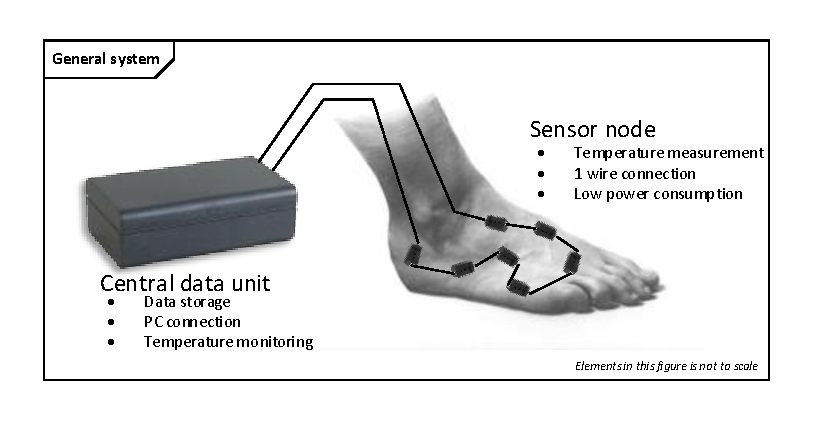
\includegraphics[width=.9\textwidth]{billeder/7requirementspec/GeneralSystem}
	\caption{Project system}
	\label{fig:project_system}
\end{figure}

The system will be mounted on and around the foot of a person who is likely to develop charcot foot. 

\section{Functionality requirements}
The sensor system has two main functionalities:
\begin{enumerate}
	\item Run in normal mode
	\item Extract captured data
\end{enumerate}

\begin{figure}[H]
	\centering
	\includegraphics[width=.7\textwidth]{billeder/7requirementspec/usecase_vector}
	\caption{Use case diagram}
\end{figure}


\section{General requirements}
\textit{This section seeks to explain the most important general requirements of the system}.
\subsection{Power consumption}

\subsection{Interface requirements}
In the central data unit requirements part of the general requirement section in the requirement specification document it is stated that the external interfaces must be:
\subsubsection{External interfaces}
\begin{table}[H]
	\begin{tabular}{p{8cm} p{2cm}}
	$\bullet$ Custom power line communication bus: & Yes\\
	$\bullet$ CDU to computer interface: & Yes\\
	\end{tabular}
\end{table}
The sensor nodes require the Custom power line communication bus as an external interface as well. These non-constricting requirements make room for a lot of different design opportunities.

\subsection{Other requirements}
